% \documentclass[10pt]{beamer}
  \documentclass[9pt]{beamer}
% \usetheme{Boadilla}
% \usetheme{default}
  \usetheme[numbering=counter]{metropolis}
  \definecolor{lightgray}{gray}{0.9}
% \definecolor{test1}{RGB}{250, 250, 230}
  \definecolor{test1}{RGB}{255, 255, 235}
  \definecolor{test2}{RGB}{240, 240, 250}
% \setbeamercolor{frametitle}{fg=black,bg=white}
  \setbeamercolor{frametitle}{fg=black,bg=test1}
  \setbeamercolor{background canvas}{bg=test2}


% acronyms for text or math mode
\newcommand {\ccast} {\mbox{\small\textsc{ccast}}}
\newcommand {\kcarta} {\mbox{k\small{CARTA}}}

\newcommand {\cris} {\mbox{\small CrIS}}
\newcommand {\airs} {\mbox{\small AIRS}}
\newcommand {\iasi} {\mbox{\small IASI}}
\newcommand {\idps} {\mbox{\small IDPS}}
\newcommand {\nasa} {\mbox{\small NASA}}
\newcommand {\noaa} {\mbox{\small NOAA}}
\newcommand {\nstar} {\mbox{\small STAR}}
\newcommand {\umbc} {\mbox{\small UMBC}}
\newcommand {\uw}   {\mbox{\small UW}}

\newcommand {\fft}  {\mbox{\small FFT}}
\newcommand {\ifft} {\mbox{\small IFFT}}
\newcommand {\fir}  {\mbox{\small FIR}}
\newcommand {\fov}  {\mbox{\small FOV}}
\newcommand {\for}  {\mbox{\small FOR}}
\newcommand {\ict}  {\mbox{\small ICT}}
\newcommand {\ils}  {\mbox{\small ILS}}
\newcommand {\igm}  {\mbox{\small IGM}}
\newcommand {\opd}  {\mbox{\small OPD}}
\newcommand {\rms}  {\mbox{\small RMS}}
\newcommand {\zpd}  {\mbox{\small ZPD}}
\newcommand {\ppm}  {\mbox{\small PPM}}
\newcommand {\srf}  {\mbox{\small SRF}}
\newcommand {\sdr}  {\mbox{\small SDR}}
\newcommand {\FWHM} {\mbox{\small FWHM}}
\newcommand {\fwhm} {\mbox{\small\textsc{fwhm}}}

\newcommand {\ES} {\mbox{\small ES}}
\newcommand {\SP} {\mbox{\small SP}}
\newcommand {\IT} {\mbox{\small IT}}
\newcommand {\SA} {\mbox{\small SA}}

\newcommand {\ET} {\mbox{\small ET}}
\newcommand {\FT} {\mbox{\small FT}}

\newcommand {\wn} {\mbox{cm$^{-1}$}}
\newcommand {\cm} {\mbox{cm}}

% abbreviations, mainly for math mode
\newcommand {\real} {\mbox{real}}
\newcommand {\imag} {\mbox{imag}}
\newcommand {\atan} {\mbox{atan}}
\newcommand {\obs}  {\mbox{obs}}
\newcommand {\calc} {\mbox{calc}}
\newcommand {\sinc} {\mbox{sinc}}
\newcommand {\psinc} {\mbox{psinc}}
\newcommand {\std} {\mbox{std}}

% symbols, for math mode only
\newcommand {\lmax} {L_{\mbox{\tiny max}}}
\newcommand {\vmax} {V_{\mbox{\tiny max}}}

\newcommand {\tauobs} {\tau_{\mbox{\tiny obs}}}
\newcommand {\taucal} {\tau_{\mbox{\tiny calc}}}
\newcommand {\Vdc}  {V_{\mbox{\tiny DC}}}

\newcommand {\rIT} {r_{\mbox{\tiny\textsc{ict}}}}
\newcommand {\rES} {r_{\mbox{\tiny\textsc{es}}}}
\newcommand {\robs} {r_{\mbox{\tiny obs}}}

\newcommand {\rITobs} {r_{\mbox{\tiny\textsc{ict}}}^{\mbox{\tiny obs}}}
\newcommand {\rITcal} {r_{\mbox{\tiny\textsc{ict}}}^{\mbox{\tiny cal}}}

\newcommand {\rESuser} {r_{\mbox{\tiny\textsc{es}}}^{\mbox{\tiny user}}}
\newcommand {\rITuser} {r_{\mbox{\tiny\textsc{ict}}}^{\mbox{\tiny user}}}
\newcommand {\rITsensor} {r_{\mbox{\tiny\textsc{ict}}}^{\mbox{\tiny sensor}}}
\newcommand {\rITfov} {r_{\mbox{\tiny\textsc{ict}}}^{\mbox{\tiny fov}}}

\newcommand {\fcos} {f_{\mbox{\tiny cos}}}
\newcommand {\fatbd} {f_{\mbox{\tiny\textsc{atbd}}}}

\newcommand {\ITmean} {\langle\mbox{\small IT}\rangle}
\newcommand {\SPmean} {\langle\mbox{\small SP}\rangle}

\newcommand {\Ttc} {t^{\mbox{\tiny\textsc{tc}}}}
\newcommand {\Tac} {t^{\mbox{\tiny\textsc{ac}}}}
\newcommand {\rtc} {r_{\mbox{\tiny\textsc{tc}}}}
\newcommand {\rta} {r_{\mbox{\tiny\textsc{ta}}}}



\title{Feb 2020 CrIS J2 TVAC MN Gas Cell ILS Tests}
\author{H.~E.~Motteler, L.~L.~Strow, \\
  S.~DeSouza-Machado, \\
  S.~Buczkowski
}
\institute{
  UMBC Atmospheric Spectroscopy Lab \\
  Joint Center for Earth Systems Technology \\
}
\date{\today}
\begin{document}

%----------- slide --------------------------------------------------%
\begin{frame}[plain]
\titlepage
\end{frame}
%----------- slide --------------------------------------------------%
\begin{frame}
\frametitle{Introduction}
\begin{itemize}

  \item We present an analysis of the CrIS J2 TVAC MN Plateau 22
    CO$_2$, CH$_4$, and CO gas cell ILS tests, and compare
    measurements with calculated reference truth from LBLRTM and
    UMBC-LBL.

  \item Overall the results look good, with metrology laser
    residuals consistent across temperature plateaus, sides, and
    bands.

  \item Examples of monitoring test logs (the CSS, CMD, and TCR
    files) are given in the form of plots of HTBB temperature, gas
    cell temperature, and gas cell pressure over time.  We did not
    have high-level logs for all tests, at the time of this
    analysis.

  \item The J2 MN tests were done at the 876/1052/808 point extended
    resolution, vs. the 866/1052/799 point high resolution used for
    PFL and PFH.

\end{itemize}
\end{frame}
%----------- slide --------------------------------------------------%
\begin{frame}
\frametitle{Methods}
\begin{itemize}

  \item For each test we partition the data into four legs, FT1,
    FT2, ET1, and ET2 (cell full, HTBB temperature T1, etc.)

  \item For each test leg, we take the mean of the associated count
    spectra, calculate the transmittance as $(FT2 - FT1) / (ET2 -
    ET1)$, apply our standard processing filters, and do the SA
    correction, all at the sensor grid.  Expected transmittance
    values are also calculated at the sensor grid.

  \item This is similar in some ways to the ``ratio first''
    calibration algorithm used as an option in UMBC CCAST
    processing, but note that we do not do a full radiance
    calibration, or any nonlinearity correction, for the analysis
    here.

  \item Measured and calculated transmittances are compared first as
    is, and then by fitting obs to calcs and examining fitting
    weights and residuals.

  \item This approach, with fitting adjustments, is acceptable for
    our application because our main task is spectral calibration
    and our fitting methods are robust in the face of radiometric
    uncertainty.

\end{itemize}
\end{frame}
%----------- slide --------------------------------------------------%
\begin{frame}
\frametitle{5 Feb 2020 TVAC MN Side 2 Plateau 22}
\begin{columns}[t]
\begin{column}{0.6\textwidth}
  \begin{centering}
  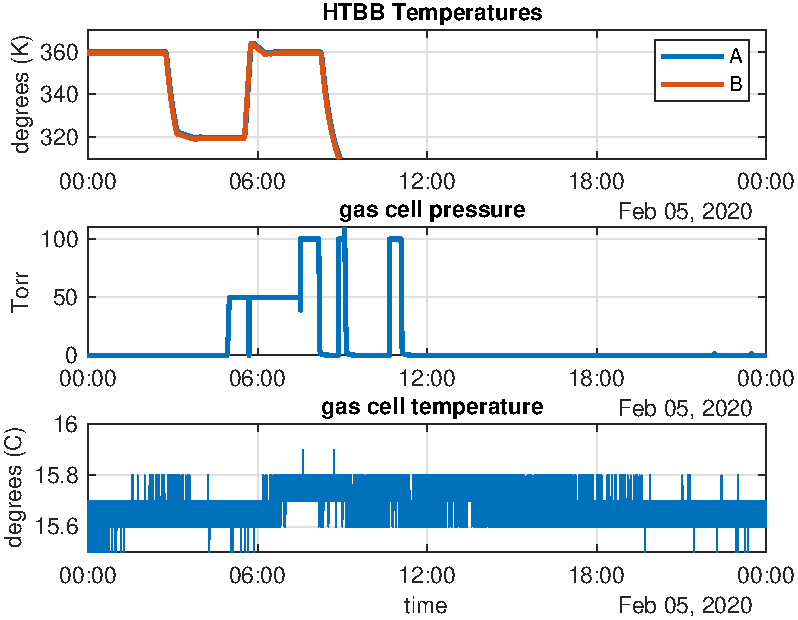
\includegraphics[width=\textwidth]{harvest_02-05/css_summary_02_05.pdf}
  \end{centering}\vspace{3mm}

% \end{column}
% \begin{column}{0.5\textwidth}  
%   \begin{centering}
%   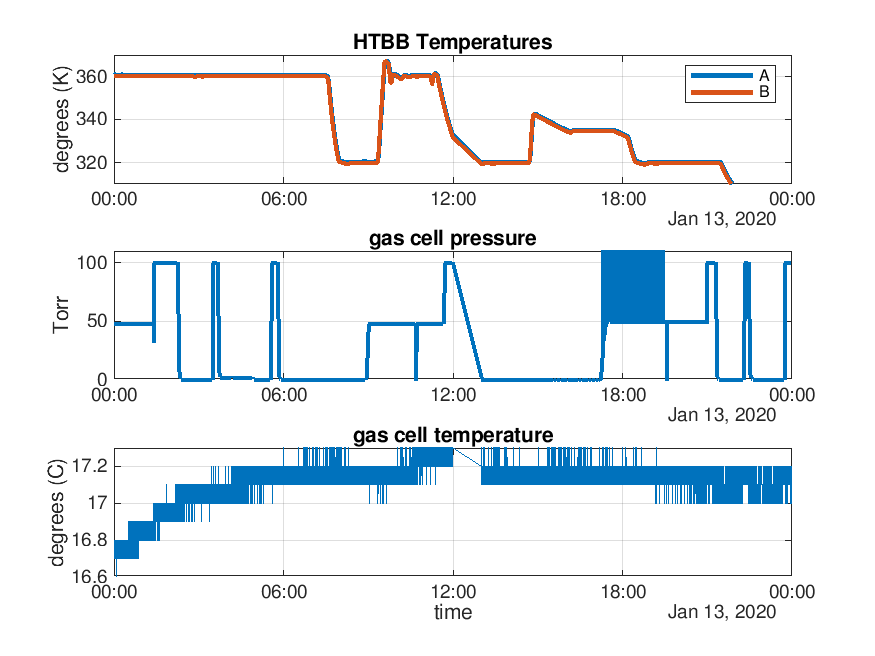
\includegraphics[width=\textwidth]{harvest_01-12/css_summary_13_jan.png}
%   \end{centering}\vspace{3mm}

\end{column}
\end{columns}

HTBB temperatures, gas cell pressure and gas cell temperature from
the CCS files, for 5 Feb 2020.  This data is used along with a scan
of the CMD and SQL files for an overview and to find the test stages.

\end{frame}
%----------- slide --------------------------------------------------%
\begin{frame}
\frametitle{CO$_2$ MN side 2 gas cell test legs}

\begin{columns}[t]
\begin{column}{0.45\textwidth}
  \begin{centering}
  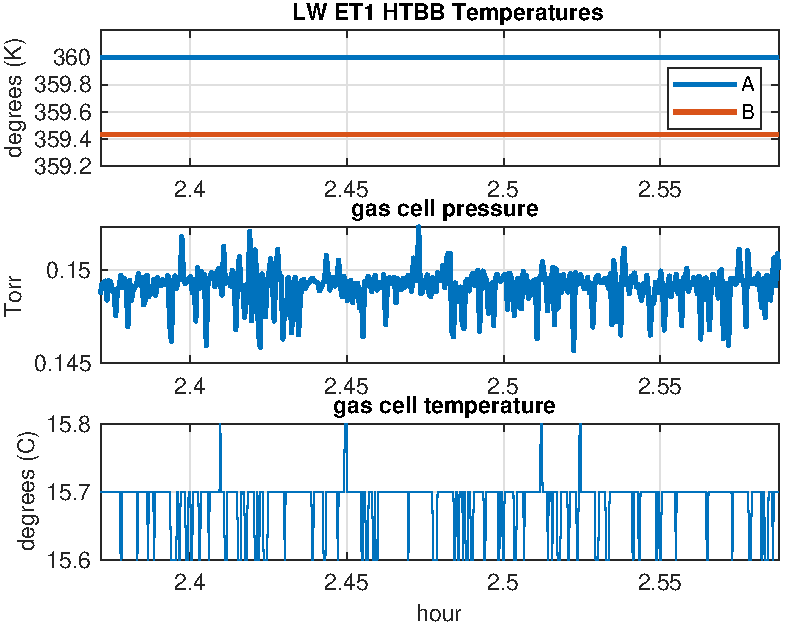
\includegraphics[width=\textwidth]{harvest_02-05/02-05_LW_ET1.pdf}
  \end{centering}
\end{column}
\begin{column}{0.45\textwidth}  
  \begin{centering}
  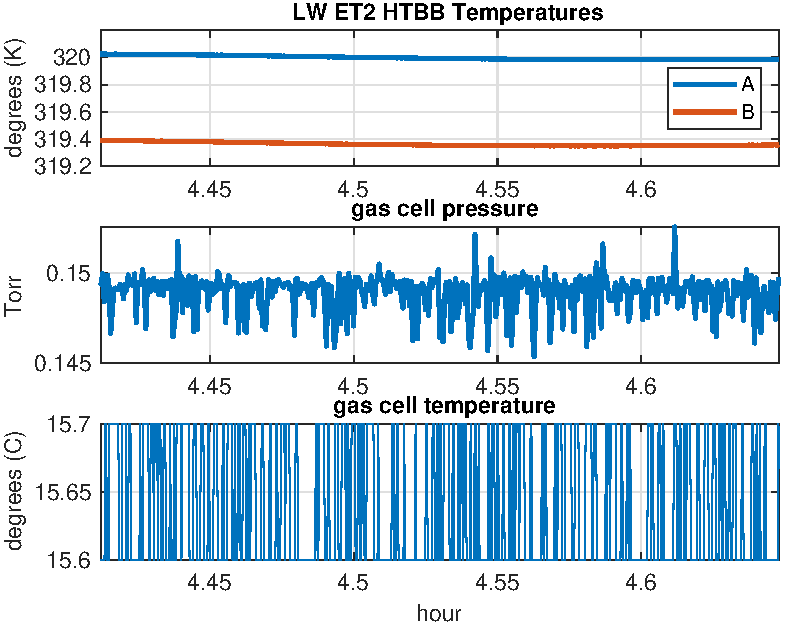
\includegraphics[width=\textwidth]{harvest_02-05/02-05_LW_ET2.pdf}
  \end{centering}
\end{column}
\end{columns}
\vspace{3mm}

\begin{columns}[t]
\begin{column}{0.45\textwidth}
  \begin{centering}
  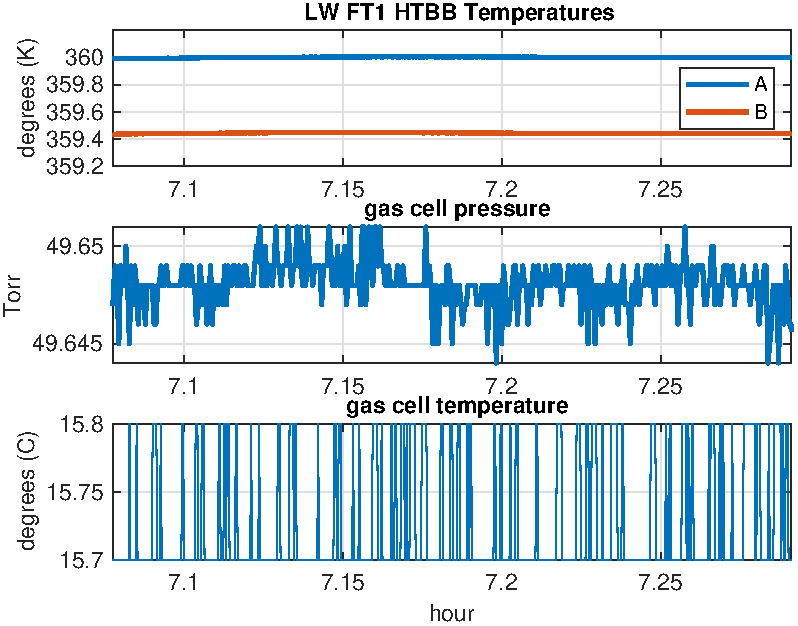
\includegraphics[width=\textwidth]{harvest_02-05/02-05_LW_FT1.pdf}
  \end{centering}
\end{column}
\begin{column}{0.45\textwidth}  
  \begin{centering}
  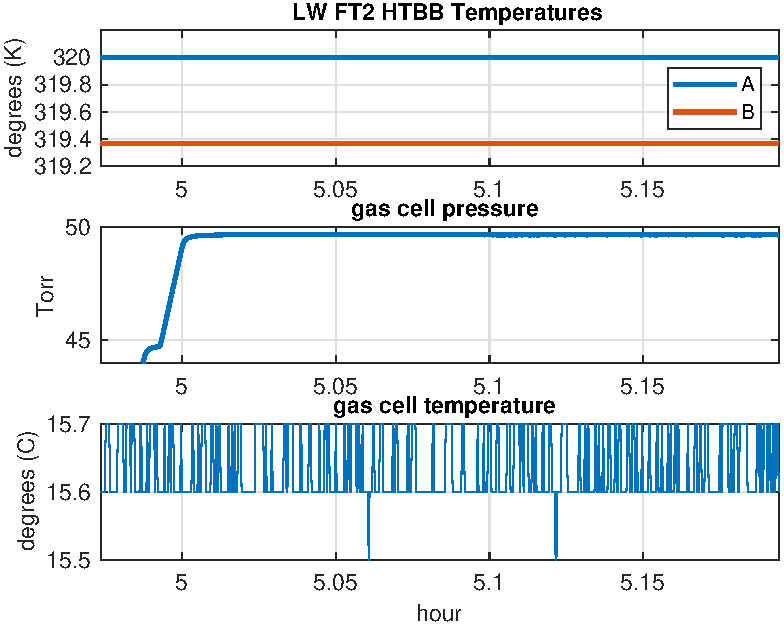
\includegraphics[width=\textwidth]{harvest_02-05/02-05_LW_FT2.pdf}
  \end{centering}
\end{column}
\end{columns}
\end{frame}
%----------- slide --------------------------------------------------%
\begin{frame}
\frametitle{CO$_2$ LW MN side 2 test parameters}

\begin{itemize}
  \item MN Plateau 22, 5 Feb 2020
  \item side 2, sweep direction 0
  \item fitting interval 672 to 712 $\wn$
  \item metrology laser 773.98002 nm, from neon 703.44765 nm
  \item ATBD default focal plane
  \item SA correction from ILS with periodic sinc at the sensor grid
  \item HTBB nominal T1 360 K, T2 320 K
  \item gas cell pressure 49.43 Torr
  \item gas cell temperature 15.60 C
  \item gas cell length 12.59 cm
\end{itemize}

\end{frame}
%----------- slide --------------------------------------------------%
\begin{frame}
\frametitle{CO$_2$ side 2 data before fitting}
\begin{columns}[t]
\begin{column}{0.5\textwidth}  
  \begin{centering}
  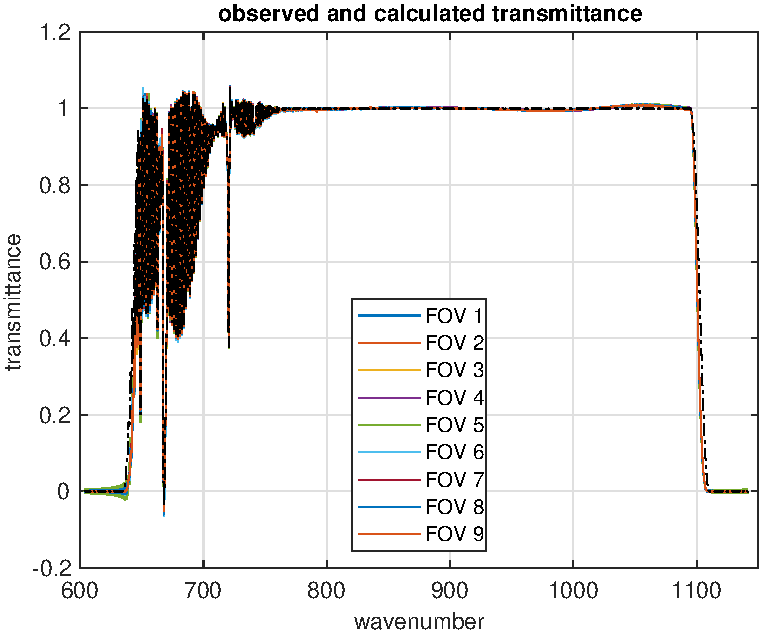
\includegraphics[width=\textwidth]{02-05_mn_s2_CO2/spec_test2_all.pdf}
  \end{centering}\vspace{3mm}

Measured transmittance after the \\ SA correction but before any
fitting, together with calculated transmittance.

\end{column}

\begin{column}{0.5\textwidth}
  \begin{centering}
  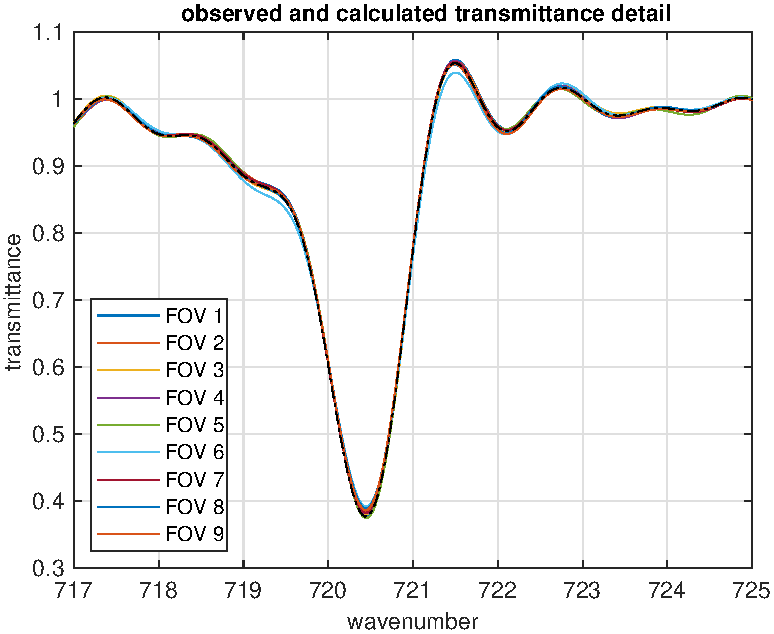
\includegraphics[width=\textwidth]{02-05_mn_s2_CO2/spec_test2_zoom.pdf}
  \end{centering}\vspace{3mm}

A detail from the previous plot.  Measured FOV to FOV consistency \\
and agreement with calculated transmittance is relatively good.

\end{column}
\end{columns}
\end{frame}
%----------- slide --------------------------------------------------%
\begin{frame}
\frametitle{CO$_2$ side 2 fitting overview}
\begin{columns}[t]
\begin{column}{0.5\textwidth}  
  \begin{centering}
  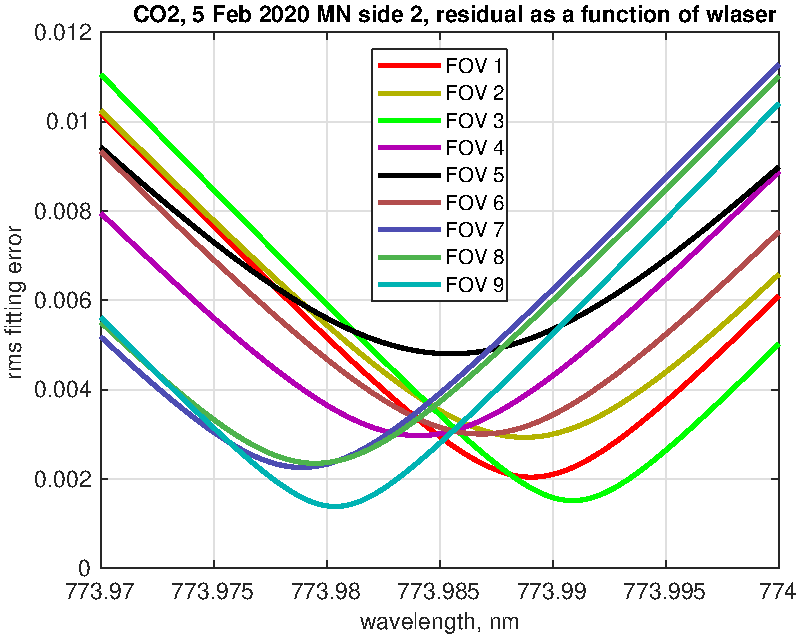
\includegraphics[width=\textwidth]{02-05_mn_s2_CO2/CO2_wlaser_fit.pdf}
  \end{centering}\vspace{3mm}

Residuals $\rms(a\cdot\tauobs + b - \taucal)$ \\ over the fitting
interval as a function \\ of metrology laser wavelength.

\end{column}

\begin{column}{0.5\textwidth}
  \begin{centering}
  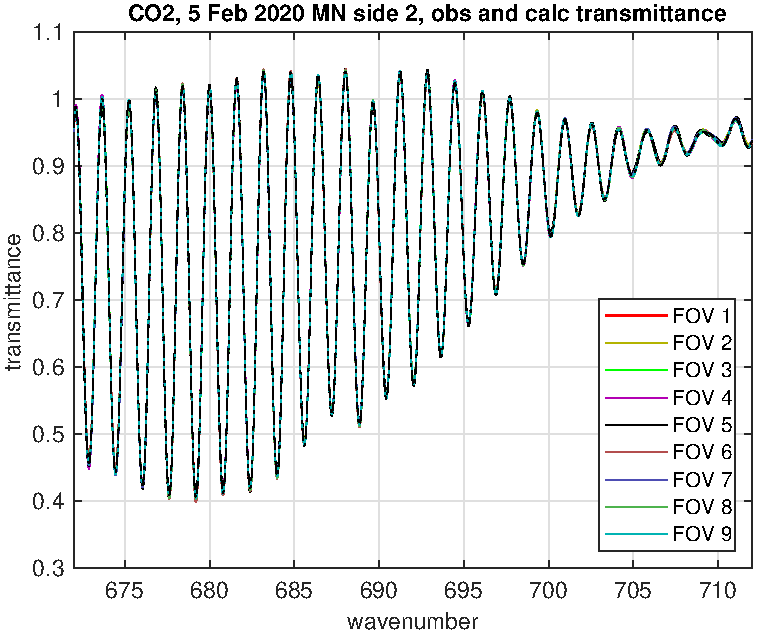
\includegraphics[width=\textwidth]{02-05_mn_s2_CO2/CO2_obs_and_calc.pdf}
  \end{centering}\vspace{3mm}

Fitted observed and calculated transmittance, over the fitting
interval.  At this level of detail we see all values are very close.

\end{column}
\end{columns}
\end{frame}
%----------- slide --------------------------------------------------%
\begin{frame}
\frametitle{CO$_2$ side 2 obs minus calc breakouts}
\begin{columns}[t]
\begin{column}{0.5\textwidth}
  \begin{centering}
  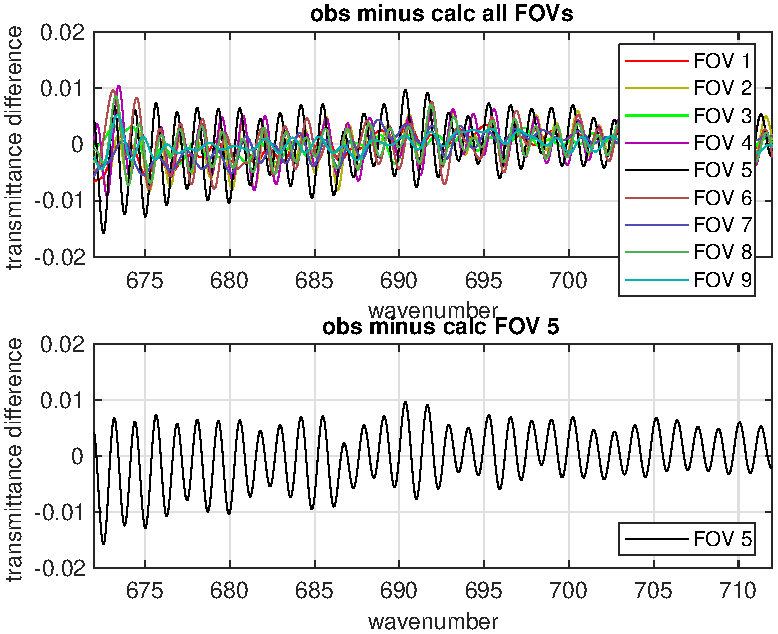
\includegraphics[width=\textwidth]{02-05_mn_s2_CO2/CO2_breakout_1.pdf}
  \end{centering}\vspace{3mm}

Fitted observed minus calculated transmittance for all FOVs and for FOV~5
alone, over the fitting interval.

\end{column}
\begin{column}{0.5\textwidth}  
  \begin{centering}
  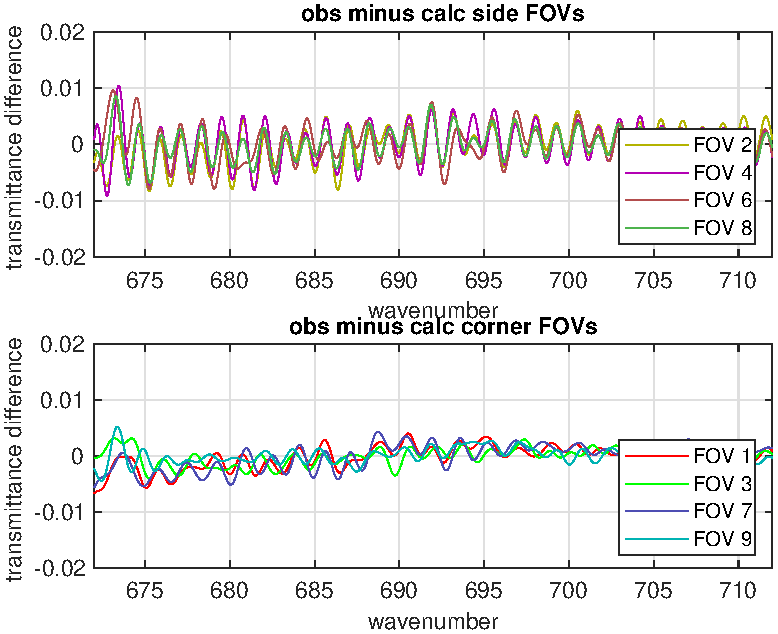
\includegraphics[width=\textwidth]{02-05_mn_s2_CO2/CO2_breakout_2.pdf}
  \end{centering}\vspace{3mm}

Fitted observed minus calculated transmittance for side and corner FOVs,
over the fitting interval.

\end{column}
\end{columns}
\end{frame}
%----------- slide --------------------------------------------------%
\begin{frame}[fragile]
\frametitle{CO$_2$ side 2 tabulated residuals}

  metrology laser absolute residuals, ppm
\begin{semiverbatim}\scriptsize
     -1.42     5.17    11.63         7   4   1
     -0.78     7.11    11.24         8   5   2
      0.52     8.91    14.08         9   6   3
\end{semiverbatim}

  metrology laser relative residuals, ppm
\begin{semiverbatim}\scriptsize
     -8.53    -1.94     4.52         7   4   1
     -7.88     0.00     4.13         8   5   2
     -6.59     1.81     6.98         9   6   3
\end{semiverbatim}

  regression fitting weights and residuals
\begin{semiverbatim}\scriptsize
 FOV   "a"       "b"     dmin     wmin      wfov
  1   0.993    0.0059   0.0020    11.63   773.9890 
  2   0.993    0.0070   0.0029    11.24   773.9887 
  3   0.991    0.0079   0.0015    14.08   773.9909 
  4   0.984    0.0140   0.0030     5.17   773.9840 
  5   0.994    0.0065   0.0048     7.11   773.9855 
  6   0.987    0.0123   0.0030     8.91   773.9869 
  7   1.002   -0.0010   0.0023    -1.42   773.9789 
  8   0.988    0.0105   0.0023    -0.78   773.9794 
  9   0.988    0.0102   0.0014     0.52   773.9804 
\end{semiverbatim}

\end{frame}
%----------- slide --------------------------------------------------%
\begin{frame}
\frametitle{11-12 Feb 2020 TVAC MN Side 1 Plateau 22}
\begin{columns}[t]
\begin{column}{0.5\textwidth}
  \begin{centering}
  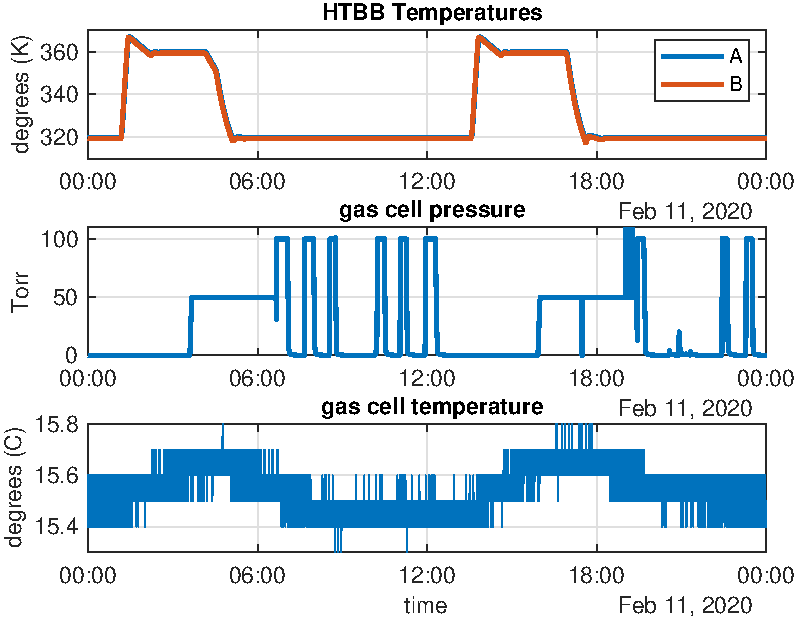
\includegraphics[width=\textwidth]{harvest_02-11/css_summary_02_11.pdf}
  \end{centering}\vspace{3mm}

\end{column}
\begin{column}{0.5\textwidth}  
  \begin{centering}
  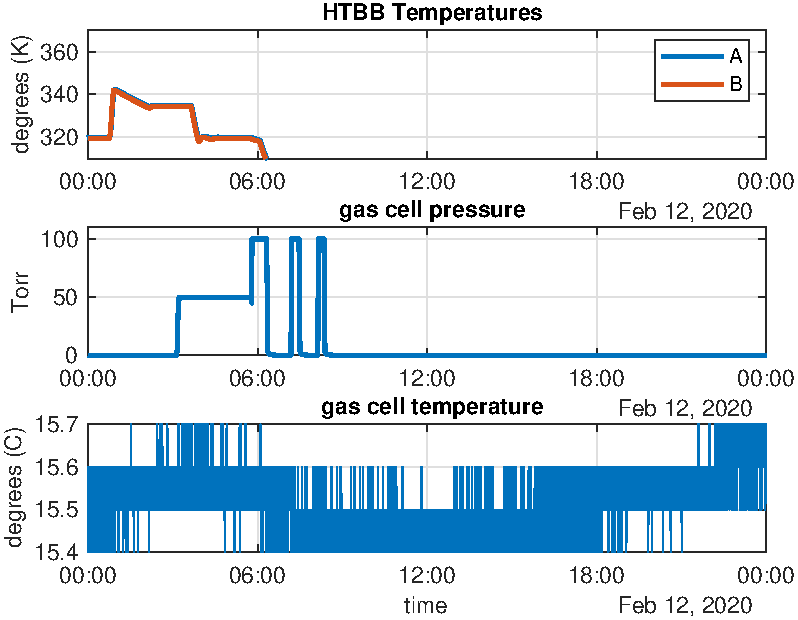
\includegraphics[width=\textwidth]{harvest_02-11/css_summary_02_12.pdf}
  \end{centering}\vspace{3mm}

\end{column}
\end{columns}

HTBB temperatures, gas cell pressure and gas cell temperature from
the CCS files, for 11-12 Feb 2020.  This data is used along with a
scan of the CMD and SQL files for an overview and to find the test
stages. 

\end{frame}
%----------- slide --------------------------------------------------%
\begin{frame}
\frametitle{CO$_2$ MN side 1 gas cell test legs}

\begin{columns}[t]
\begin{column}{0.45\textwidth}
  \begin{centering}
  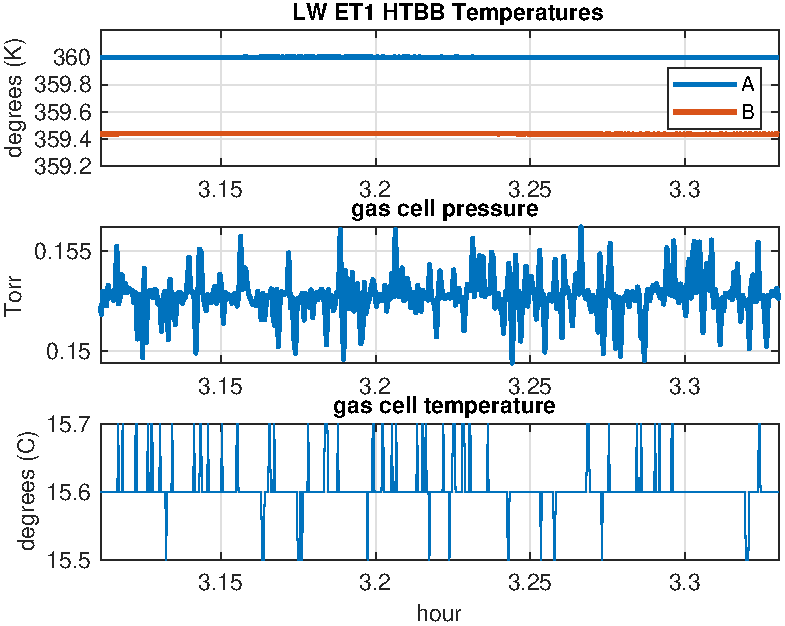
\includegraphics[width=\textwidth]{harvest_02-11/02-11_LW_ET1.pdf}
  \end{centering}
\end{column}
\begin{column}{0.45\textwidth}  
  \begin{centering}
  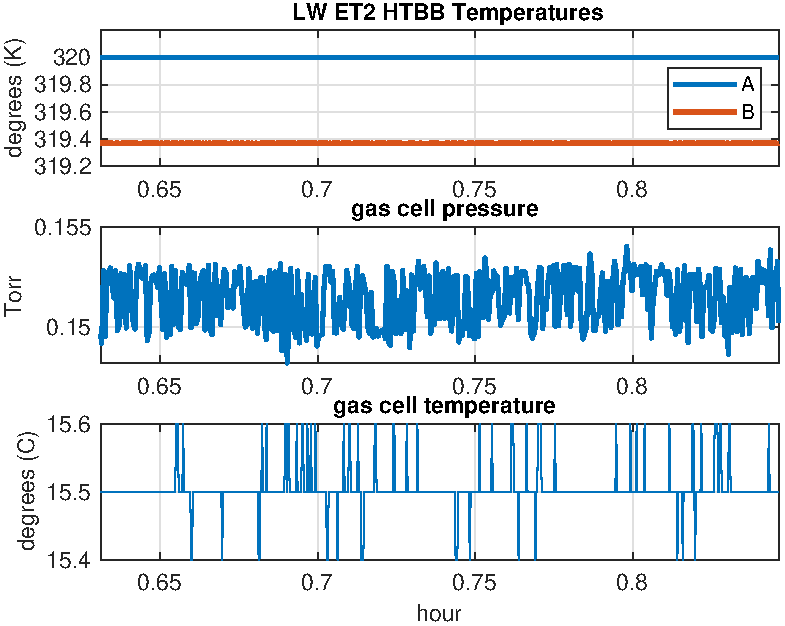
\includegraphics[width=\textwidth]{harvest_02-11/02-11_LW_ET2.pdf}
  \end{centering}
\end{column}
\end{columns}
\vspace{3mm}

\begin{columns}[t]
\begin{column}{0.45\textwidth}
  \begin{centering}
  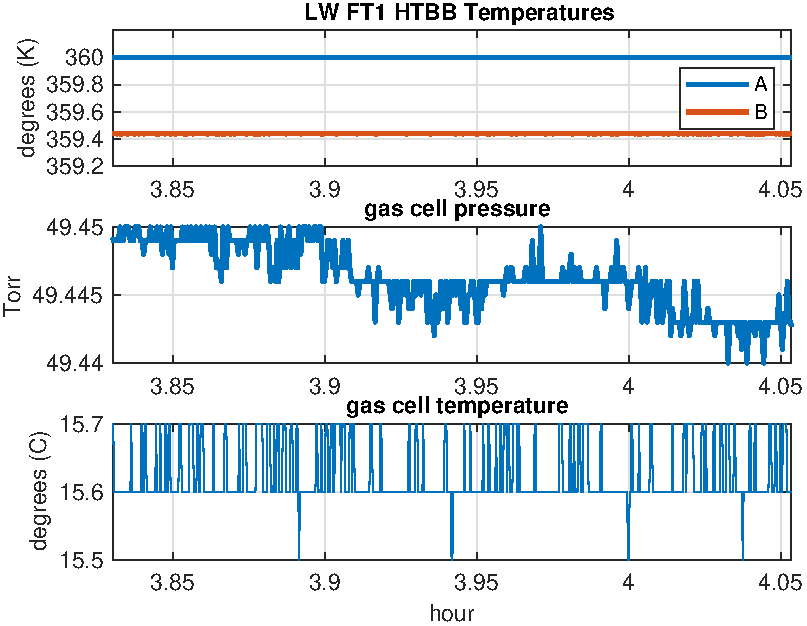
\includegraphics[width=\textwidth]{harvest_02-11/02-11_LW_FT1.pdf}
  \end{centering}
\end{column}
\begin{column}{0.45\textwidth}  
  \begin{centering}
  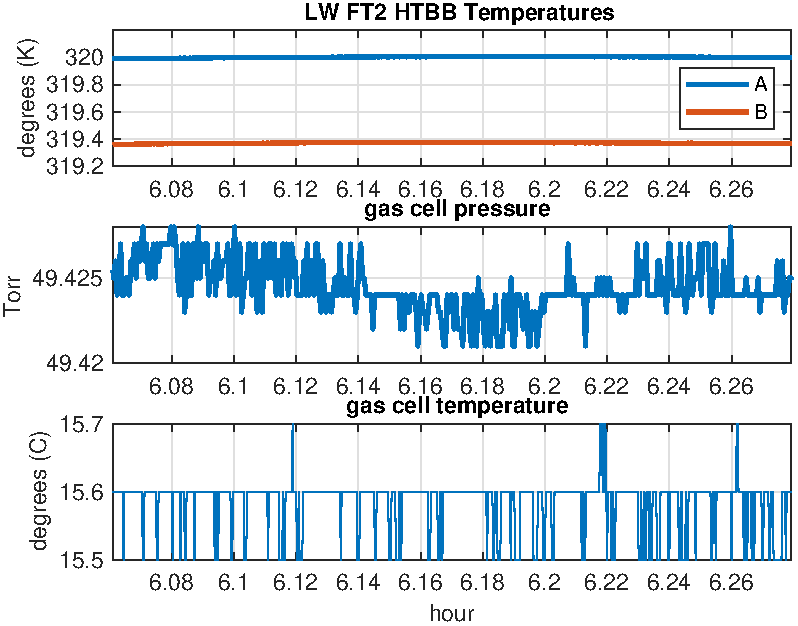
\includegraphics[width=\textwidth]{harvest_02-11/02-11_LW_FT2.pdf}
  \end{centering}
\end{column}
\end{columns}
\end{frame}
%----------- slide --------------------------------------------------%
\begin{frame}
\frametitle{CO$_2$ LW MN side 1 test parameters}

\begin{itemize}
  \item MN Plateau 22, 11 Feb 2020
  \item side 1, sweep direction 0
  \item fitting interval 672 to 712 $\wn$
  \item metrology laser 773.11974 nm, from neon 703.44765 nm
  \item ATBD default focal plane
  \item SA correction from ILS with periodic sinc at the sensor grid
  \item HTBB nominal T1 360 K, T2 320 K
  \item gas cell pressure 49.65 Torr
  \item gas cell temperature 15.70 C
  \item gas cell length 12.59 cm
\end{itemize}

\end{frame}
%----------- slide --------------------------------------------------%
\begin{frame}
\frametitle{CO$_2$ side 1 data before fitting}
\begin{columns}[t]
\begin{column}{0.5\textwidth}  
  \begin{centering}
  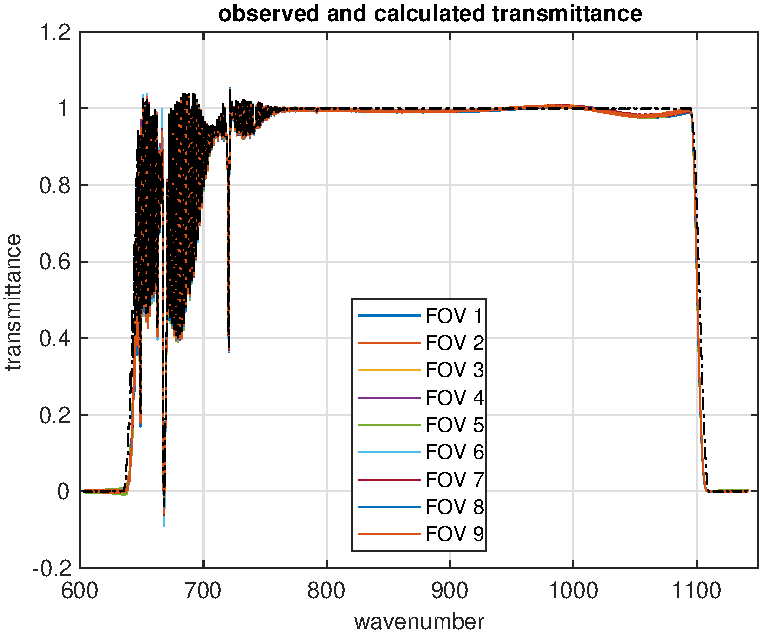
\includegraphics[width=\textwidth]{02-11_mn_s1_CO2/spec_test2_all.pdf}
  \end{centering}\vspace{3mm}

Measured transmittance after the \\ SA correction but before any
fitting, together with calculated transmittance.

\end{column}

\begin{column}{0.5\textwidth}
  \begin{centering}
  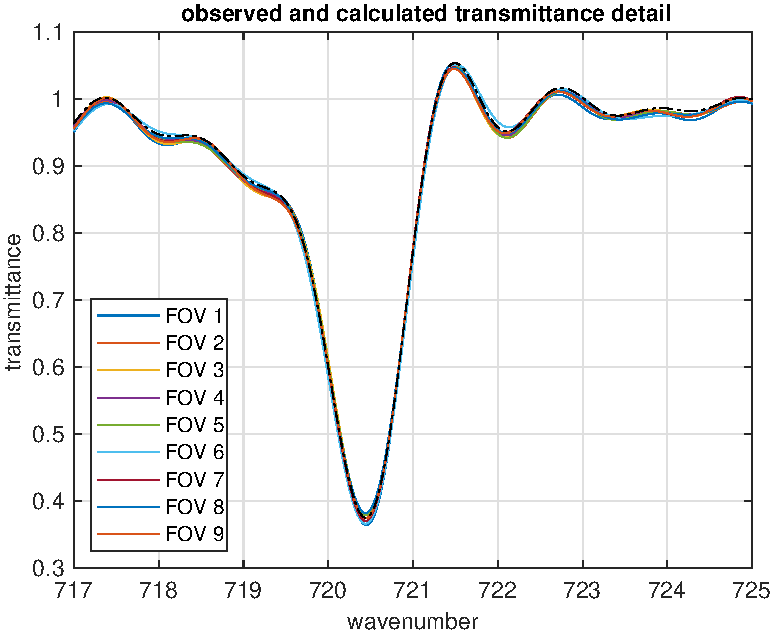
\includegraphics[width=\textwidth]{02-11_mn_s1_CO2/spec_test2_zoom.pdf}
  \end{centering}\vspace{3mm}

A detail from the previous plot.  Measured FOV to FOV consistency \\
and agreement with calculated transmittance is relatively good.

\end{column}
\end{columns}
\end{frame}
%----------- slide --------------------------------------------------%
\begin{frame}
\frametitle{CO$_2$ side 1 fitting overview}
\begin{columns}[t]
\begin{column}{0.5\textwidth}
  \begin{centering}
  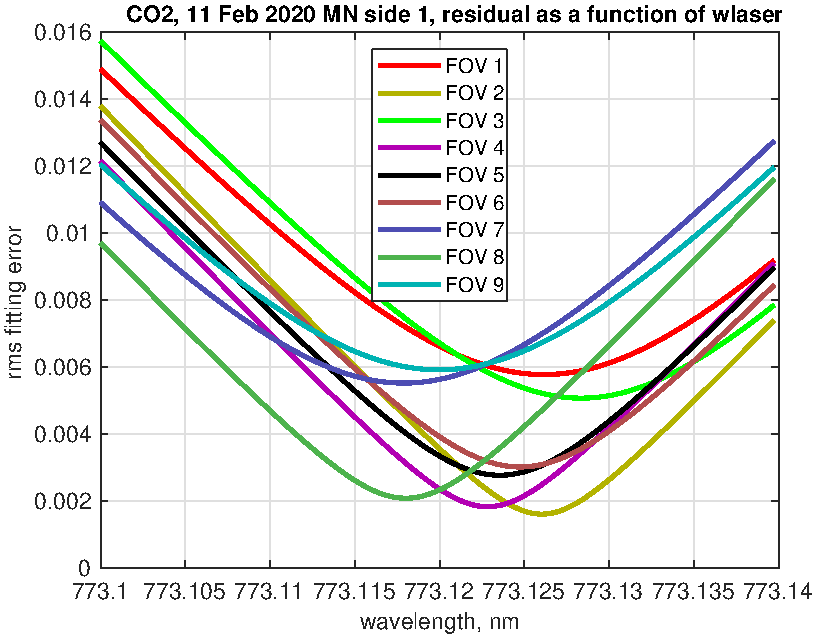
\includegraphics[width=\textwidth]{02-11_mn_s1_CO2/CO2_wlaser_fit.pdf}
  \end{centering}\vspace{3mm}

Residuals $\rms(a\cdot\tauobs + b - \taucal)$ \\ over the fitting
interval as a function \\ of metrology laser wavelength.

\end{column}
\begin{column}{0.5\textwidth}  
  \begin{centering}
  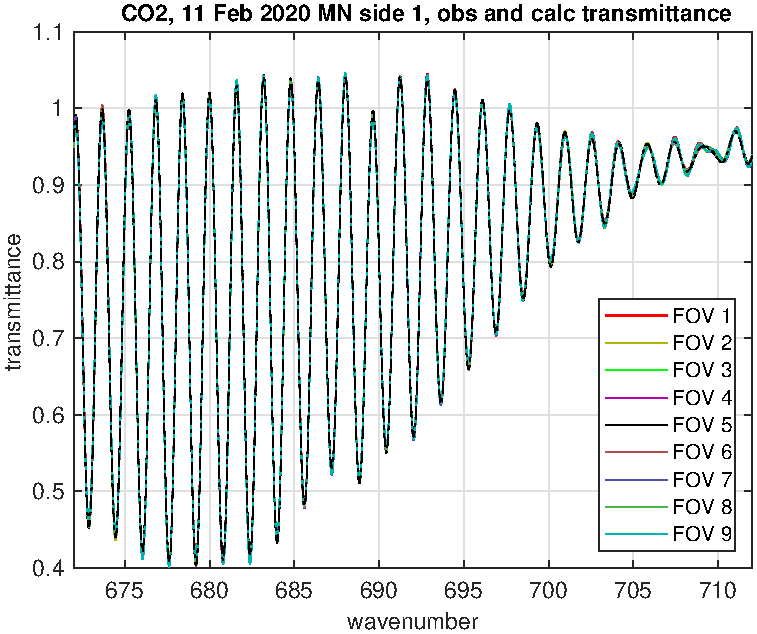
\includegraphics[width=\textwidth]{02-11_mn_s1_CO2/CO2_obs_and_calc.pdf}
  \end{centering}\vspace{3mm}

Fitted observed and calculated transmittance, over the fitting
interval.  At this level of detail we see all values are very close.

\end{column}
\end{columns}
\end{frame}
%----------- slide --------------------------------------------------%
\begin{frame}
\frametitle{CO$_2$ side 1 obs minus calc breakouts}
\begin{columns}[t]
\begin{column}{0.5\textwidth}
  \begin{centering}
  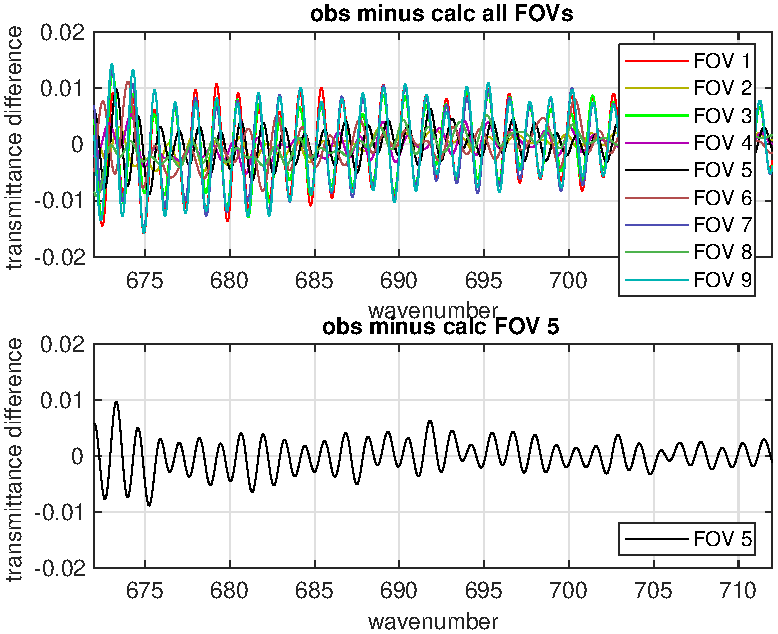
\includegraphics[width=\textwidth]{02-11_mn_s1_CO2/CO2_breakout_1.pdf}
  \end{centering}\vspace{3mm}

Fitted observed minus calculated transmittance for all FOVs and for FOV~5
alone, over the fitting interval.

\end{column}
\begin{column}{0.5\textwidth}  
  \begin{centering}
  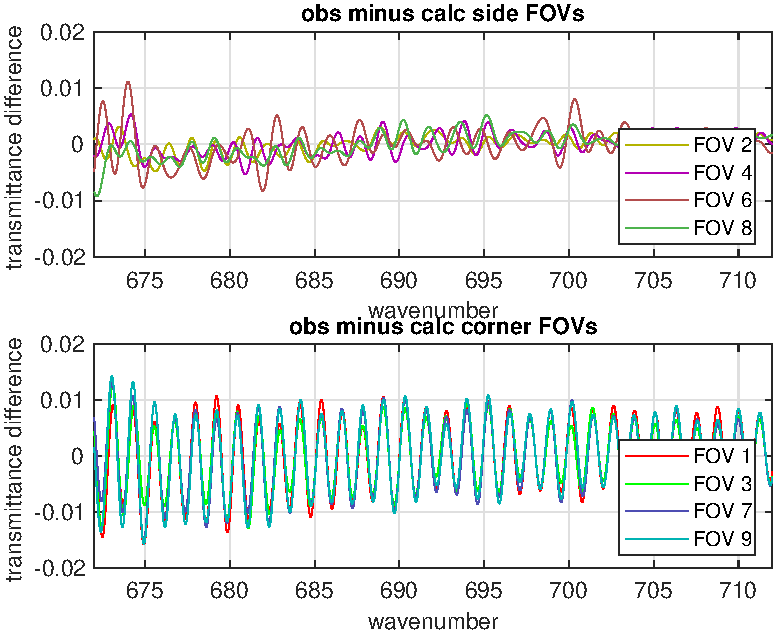
\includegraphics[width=\textwidth]{02-11_mn_s1_CO2/CO2_breakout_2.pdf}
  \end{centering}\vspace{3mm}

Fitted observed minus calculated transmittance for side and corner FOVs,
over the fitting interval.

\end{column}
\end{columns}
\end{frame}
%----------- slide --------------------------------------------------%
\begin{frame}[fragile]
\frametitle{CO$_2$ side 1 tabulated residuals}

  metrology laser absolute residuals, ppm
\begin{semiverbatim}\scriptsize
     -2.33     4.01     8.15         7   4   1
     -2.20     4.92     8.15         8   5   2
      0.39     6.47    11.12         9   6   3
\end{semiverbatim}

  metrology laser relative residuals, ppm
\begin{semiverbatim}\scriptsize
     -7.24    -0.91     3.23         7   4   1
     -7.11     0.00     3.23         8   5   2
     -4.53     1.55     6.21         9   6   3
\end{semiverbatim}

     regression fitting weights and residuals
\begin{semiverbatim}\scriptsize
 FOV   "a"       "b"     dmin     wmin      wfov
  1   1.003    0.0061   0.0058     8.15   773.1260 
  2   0.997    0.0109   0.0016     8.15   773.1260 
  3   0.996    0.0105   0.0051    11.12   773.1283 
  4   0.999    0.0094   0.0018     4.01   773.1228 
  5   0.992    0.0150   0.0028     4.92   773.1235 
  6   1.001    0.0063   0.0030     6.47   773.1247 
  7   1.003    0.0041   0.0055    -2.33   773.1179 
  8   1.005    0.0029   0.0021    -2.20   773.1180 
  9   1.005    0.0028   0.0059     0.39   773.1200 
\end{semiverbatim}

\end{frame}
%----------- slide --------------------------------------------------%
\begin{frame}
\frametitle{CH$_4$ MN side 1 gas cell test legs}

\begin{columns}[t]
\begin{column}{0.45\textwidth}
  \begin{centering}
  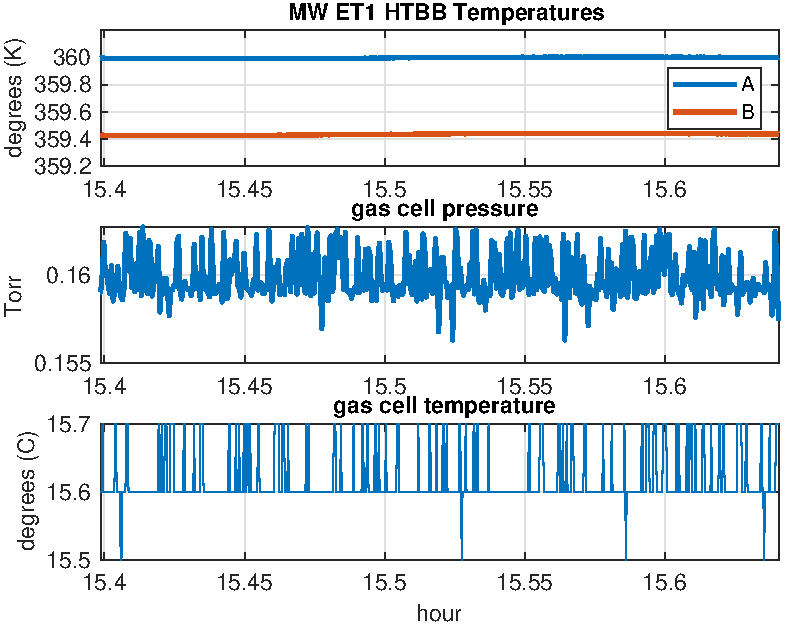
\includegraphics[width=\textwidth]{harvest_02-11/02-11_MW_ET1.pdf}
  \end{centering}
\end{column}
\begin{column}{0.45\textwidth}  
  \begin{centering}
  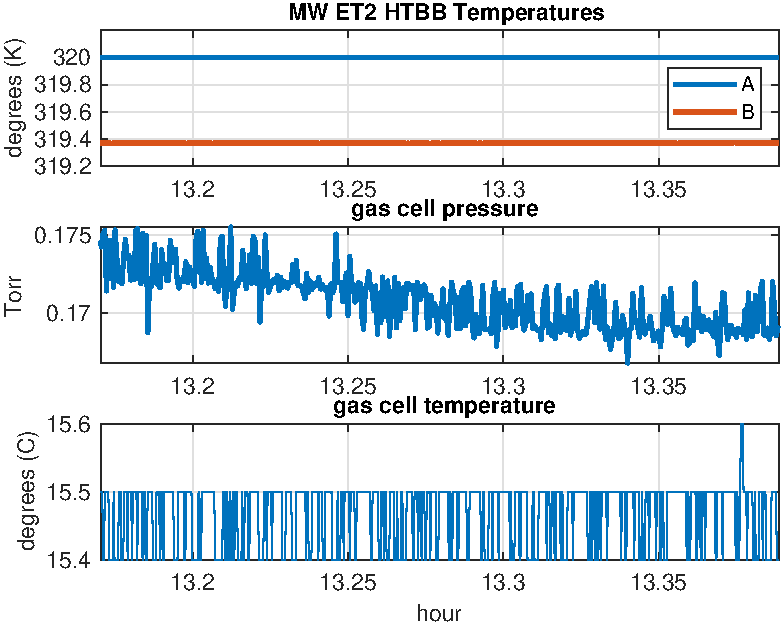
\includegraphics[width=\textwidth]{harvest_02-11/02-11_MW_ET2.pdf}
  \end{centering}
\end{column}
\end{columns}
\vspace{3mm}

\begin{columns}[t]
\begin{column}{0.45\textwidth}
  \begin{centering}
  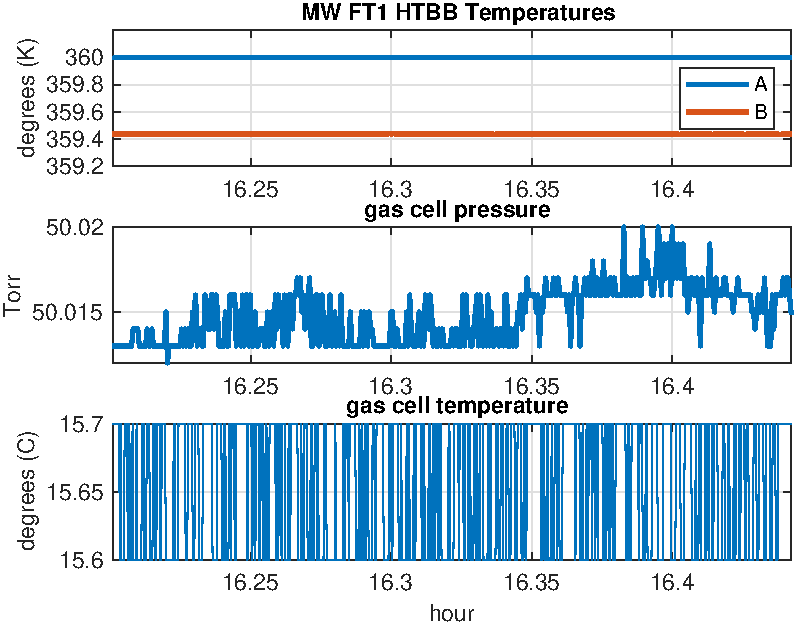
\includegraphics[width=\textwidth]{harvest_02-11/02-11_MW_FT1.pdf}
  \end{centering}
\end{column}
\begin{column}{0.45\textwidth}  
  \begin{centering}
  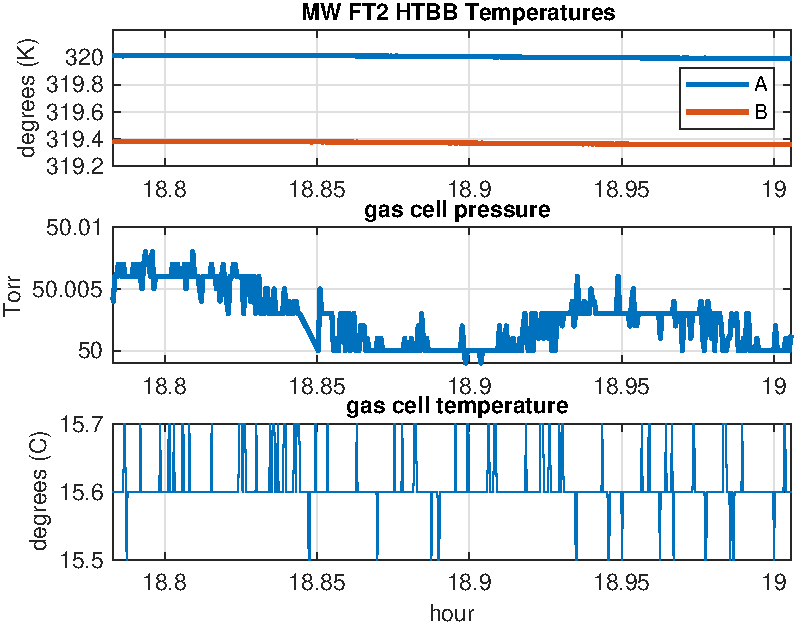
\includegraphics[width=\textwidth]{harvest_02-11/02-11_MW_FT2.pdf}
  \end{centering}
\end{column}
\end{columns}

\end{frame}
%----------- slide --------------------------------------------------%
\begin{frame}
\frametitle{CH$_4$ MW MN side 1 test parameters}

\begin{itemize}
  \item MN Plateau 22, 11 Feb 2020
  \item side 1, sweep direction 0
  \item fitting interval 1220 to 1380 $\wn$
  \item metrology laser 773.11984 nm, from neon 703.44765 nm
  \item ATBD default focal plane
  \item SA correction from ILS with periodic sinc at the sensor grid
  \item HTBB nominal T1 360 K, T2 320 K
  \item gas cell pressure 50.00 Torr
  \item gas cell temperature 15.63 C
  \item gas cell length 12.59 cm
\end{itemize}

\end{frame}
%----------- slide --------------------------------------------------%
\begin{frame}
\frametitle{CH$_4$ side 1 data before fitting}
\begin{columns}[t]
\begin{column}{0.5\textwidth}  
  \begin{centering}
  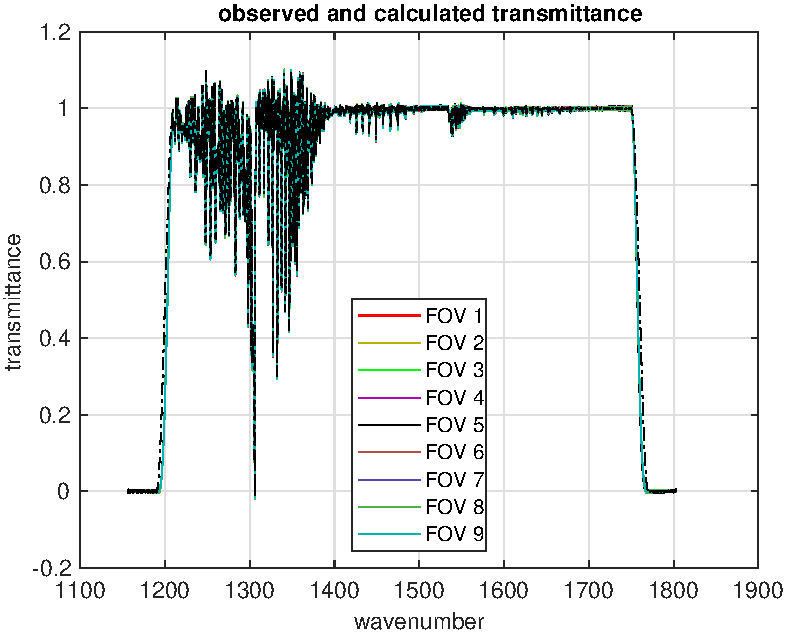
\includegraphics[width=\textwidth]{02-11_mn_s1_CH4/spec_test2_all.pdf}
  \end{centering}\vspace{3mm}

Measured transmittance after the \\ SA correction but before any
fitting, together with calculated transmittance.

\end{column}

\begin{column}{0.5\textwidth}
  \begin{centering}
  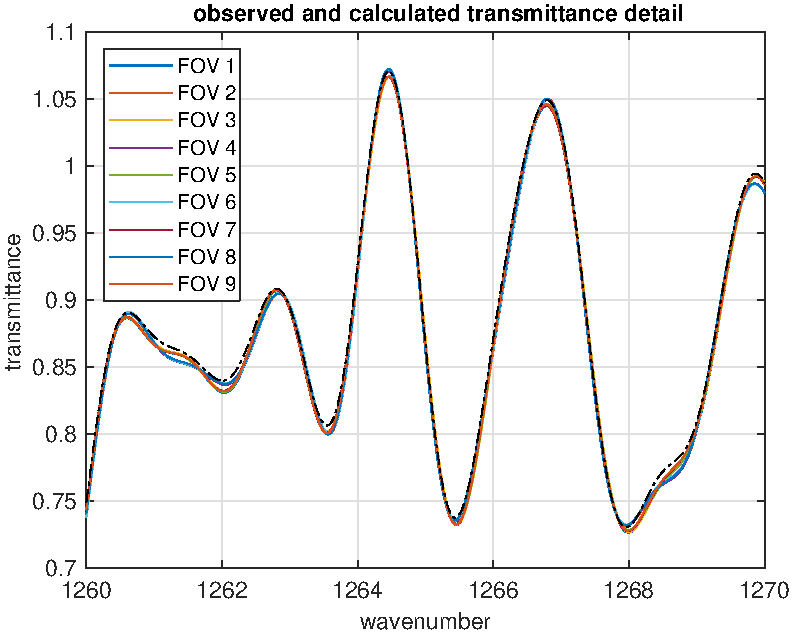
\includegraphics[width=\textwidth]{02-11_mn_s1_CH4/spec_test2_zoom.pdf}
  \end{centering}\vspace{3mm}

A detail from the previous plot.  Measured FOV to FOV consistency \\
and agreement with calculated transmittance is relatively good.

\end{column}
\end{columns}
\end{frame}
%----------- slide --------------------------------------------------%
\begin{frame}
\frametitle{CH$_4$ side 1 fitting overview}
\begin{columns}[t]
\begin{column}{0.5\textwidth}
  \begin{centering}
  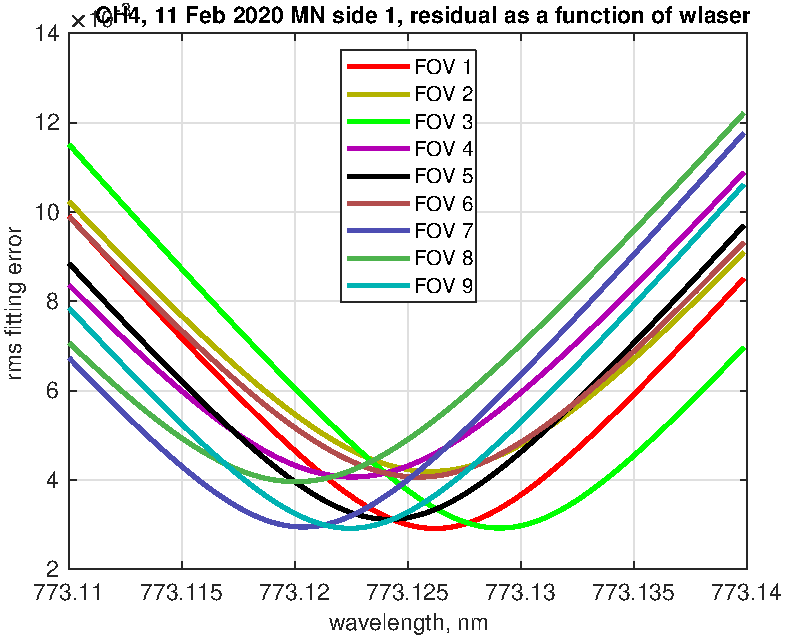
\includegraphics[width=\textwidth]{02-11_mn_s1_CH4/CH4_wlaser_fit.pdf}
  \end{centering}\vspace{3mm}

Residuals $\rms(a\cdot\tauobs + b - \taucal)$ \\ over the fitting
interval as a function \\ of metrology laser wavelength.

\end{column}
\begin{column}{0.5\textwidth}  
  \begin{centering}
  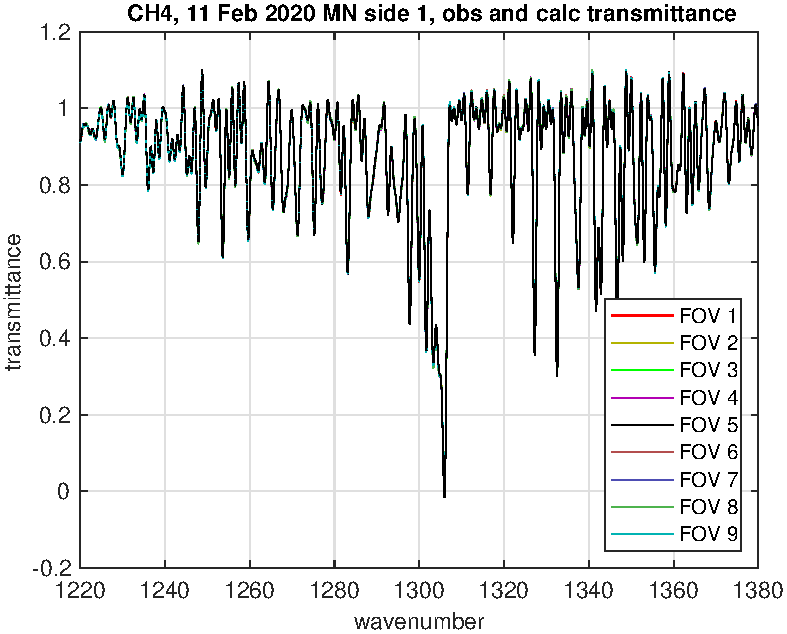
\includegraphics[width=\textwidth]{02-11_mn_s1_CH4/CH4_obs_and_calc.pdf}
  \end{centering}\vspace{3mm}

Fitted observed and calculated transmittance, over the fitting
interval.  At this level of detail we see all values are very close.

\end{column}
\end{columns}
\end{frame}
%----------- slide --------------------------------------------------%
\begin{frame}
\frametitle{CH$_4$ side 1 obs minus calc breakouts}
\begin{columns}[t]
\begin{column}{0.5\textwidth}
  \begin{centering}
  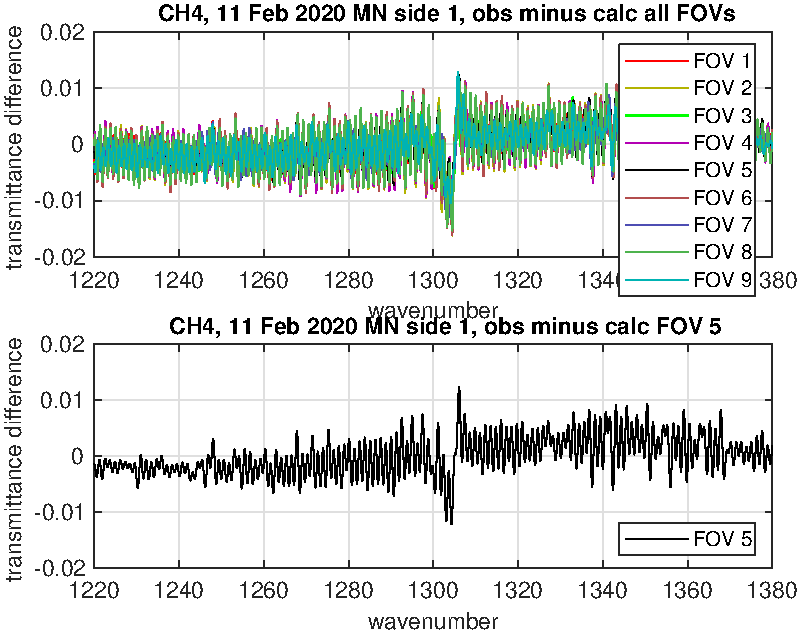
\includegraphics[width=\textwidth]{02-11_mn_s1_CH4/CH4_breakout_1.pdf}
  \end{centering}\vspace{3mm}

Fitted observed minus calculated transmittance for all FOVs and for FOV~5
alone, over the fitting interval.

\end{column}
\begin{column}{0.5\textwidth}  
  \begin{centering}
  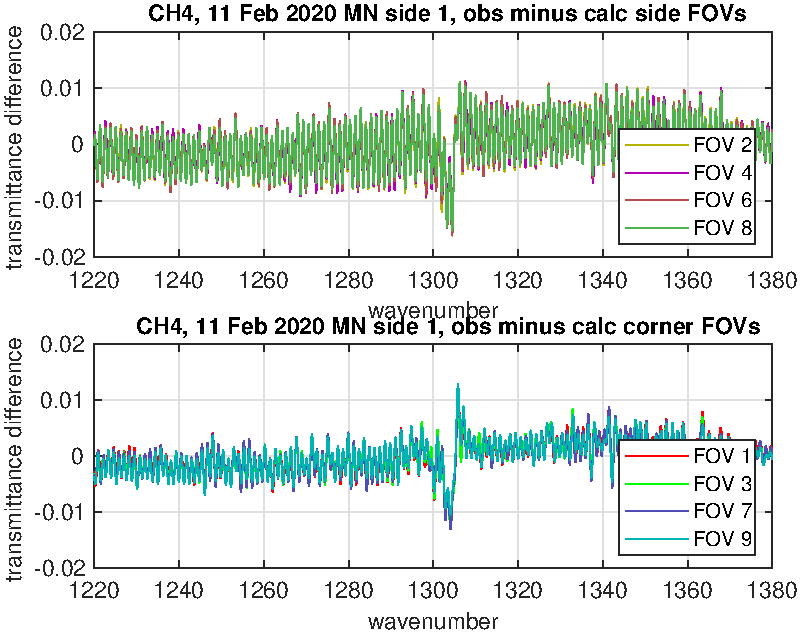
\includegraphics[width=\textwidth]{02-11_mn_s1_CH4/CH4_breakout_2.pdf}
  \end{centering}\vspace{3mm}

Fitted observed minus calculated transmittance for side and corner FOVs,
over the fitting interval.

\end{column}
\end{columns}
\end{frame}
%----------- slide --------------------------------------------------%
\begin{frame}[fragile]
\frametitle{CH$_4$ side 1 tabulated residuals}

  metrology laser absolute residuals, ppm
\begin{semiverbatim}\scriptsize
      0.65     3.49     8.15         7   4   1
      0.26     5.56     8.02         8   5   2
      3.36     7.24    11.90         9   6   3
\end{semiverbatim}

  metrology laser relative residuals, ppm
\begin{semiverbatim}\scriptsize
     -4.92    -2.07     2.59         7   4   1
     -5.30     0.00     2.46         8   5   2
     -2.20     1.68     6.34         9   6   3
\end{semiverbatim}

  regression fitting weights and residuals
\begin{semiverbatim}\scriptsize
 FOV   "a"       "b"     dmin     wmin      wfov
  1   0.986    0.0143   0.0029     8.15   773.1261 
  2   0.990    0.0109   0.0042     8.02   773.1260 
  3   0.986    0.0136   0.0029    11.90   773.1290 
  4   0.991    0.0099   0.0041     3.49   773.1225 
  5   0.988    0.0121   0.0031     5.56   773.1241 
  6   0.991    0.0094   0.0041     7.24   773.1254 
  7   0.989    0.0114   0.0029     0.65   773.1203 
  8   0.990    0.0108   0.0040     0.26   773.1200 
  9   0.989    0.0113   0.0029     3.36   773.1224 
\end{semiverbatim}

\end{frame}
%----------- slide --------------------------------------------------%
\begin{frame}
\frametitle{CO MN side gas cell test legs}

\begin{columns}[t]
\begin{column}{0.45\textwidth}
  \begin{centering}
  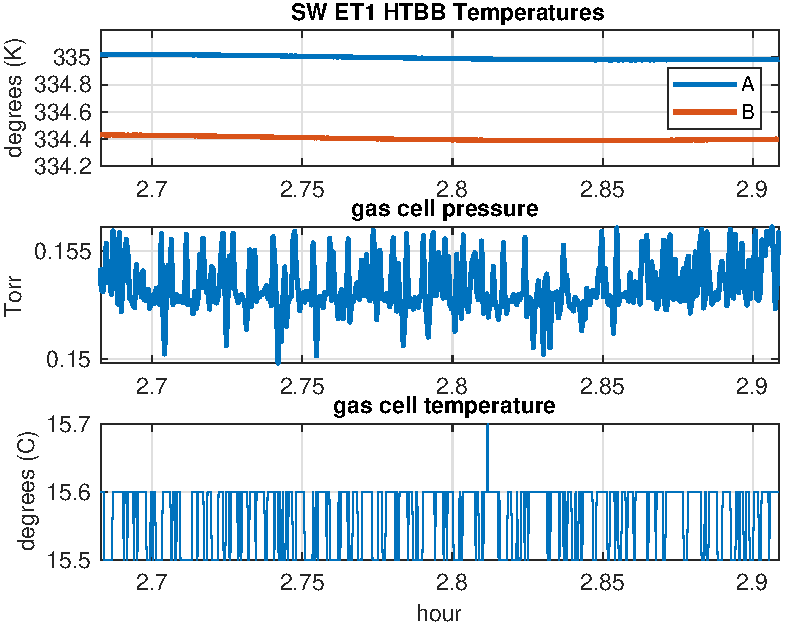
\includegraphics[width=\textwidth]{harvest_02-11/02-12_SW_ET1.pdf}
  \end{centering}
\end{column}
\begin{column}{0.45\textwidth}  
  \begin{centering}
  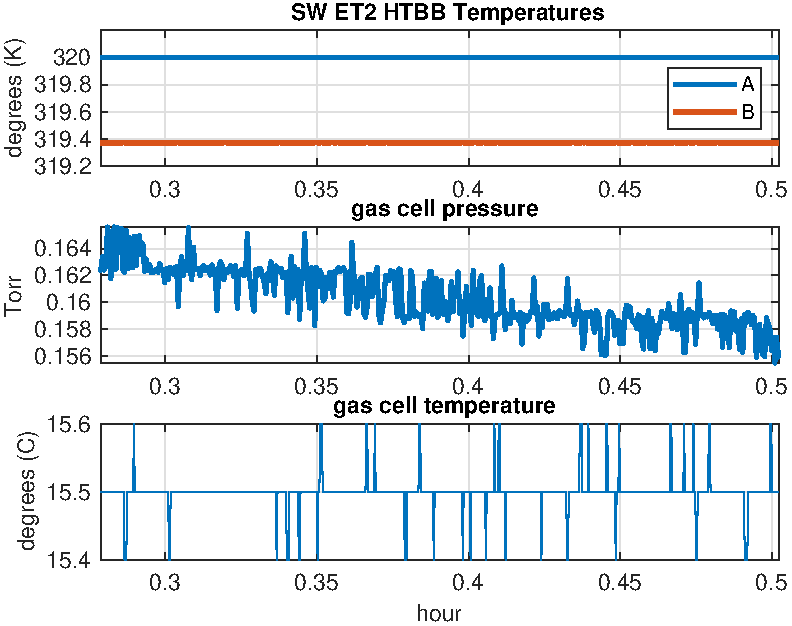
\includegraphics[width=\textwidth]{harvest_02-11/02-12_SW_ET2.pdf}
  \end{centering}
\end{column}
\end{columns}
\vspace{3mm}

\begin{columns}[t]
\begin{column}{0.45\textwidth}
  \begin{centering}
  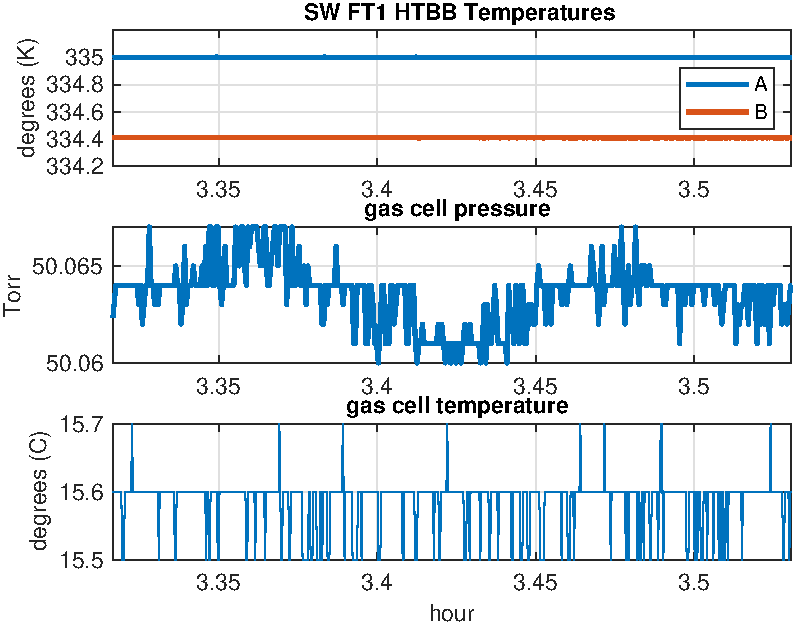
\includegraphics[width=\textwidth]{harvest_02-11/02-12_SW_FT1.pdf}
  \end{centering}
\end{column}
\begin{column}{0.45\textwidth}  
  \begin{centering}
  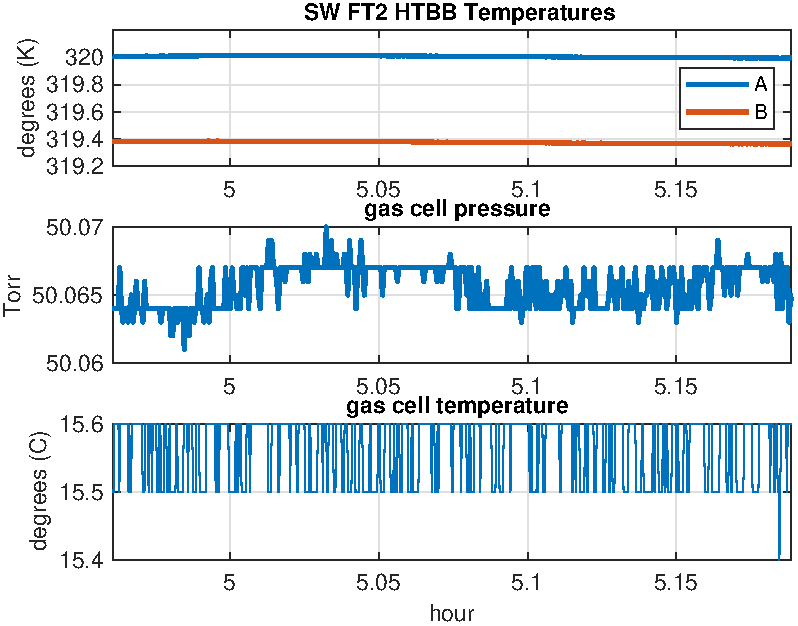
\includegraphics[width=\textwidth]{harvest_02-11/02-12_SW_FT2.pdf}
  \end{centering}
\end{column}
\end{columns}

\end{frame}
%----------- slide --------------------------------------------------%
\begin{frame}
\frametitle{CO SW MN side 1 test parameters}

\begin{itemize}
  \item MN Plateau 22, 12 Feb 2020
  \item side 1, sweep direction 0
  \item fitting interval 2160 to 2240 $\wn$
  \item metrology laser 773.11979 nm, from neon 703.44765 nm
  \item ATBD default focal plane
  \item SA correction from ILS with periodic sinc at the sensor grid
  \item HTBB nominal T1 335 K, T2 320 K
  \item gas cell pressure 50.06 Torr
  \item gas cell temperature 15.57 C
  \item gas cell length 12.59 cm
\end{itemize}

\end{frame}
%----------- slide --------------------------------------------------%
\begin{frame}
\frametitle{CO side 1 data before fitting}
\begin{columns}[t]
\begin{column}{0.5\textwidth}  
  \begin{centering}
  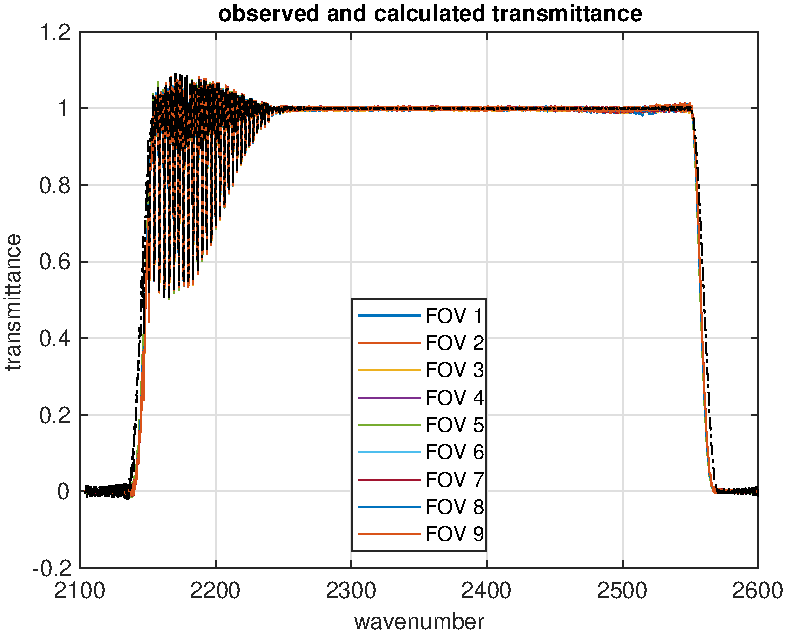
\includegraphics[width=\textwidth]{02-12_mn_s1_CO/spec_test2_all.pdf}
  \end{centering}\vspace{3mm}

Measured transmittance after the \\ SA correction but before any
fitting, together with calculated transmittance.

\end{column}

\begin{column}{0.5\textwidth}
  \begin{centering}
  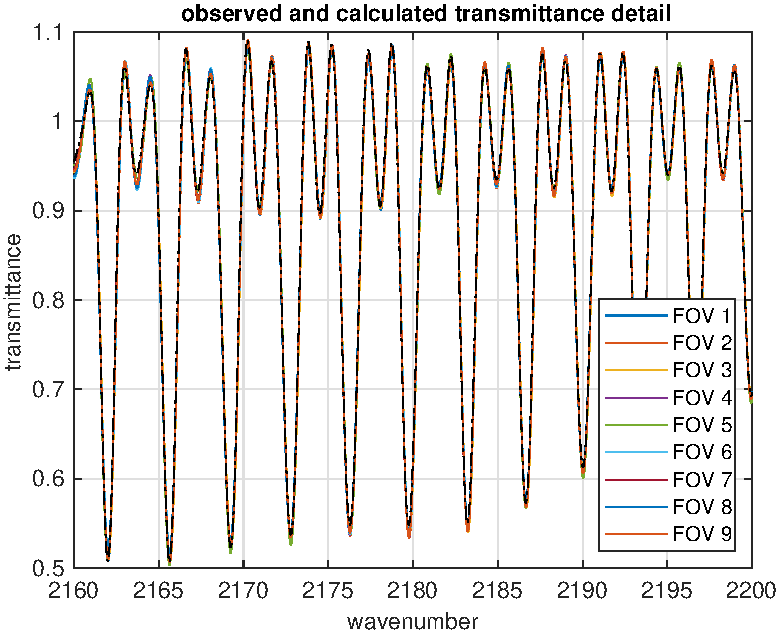
\includegraphics[width=\textwidth]{02-12_mn_s1_CO/spec_test2_zoom.pdf}
  \end{centering}\vspace{3mm}

A detail from the previous plot.  Measured FOV to FOV consistency \\
and agreement with calculated transmittance is relatively good.

\end{column}
\end{columns}
\end{frame}
%----------- slide --------------------------------------------------%
\begin{frame}
\frametitle{CO side 1 fitting overview}
\begin{columns}[t]
\begin{column}{0.5\textwidth}
  \begin{centering}
  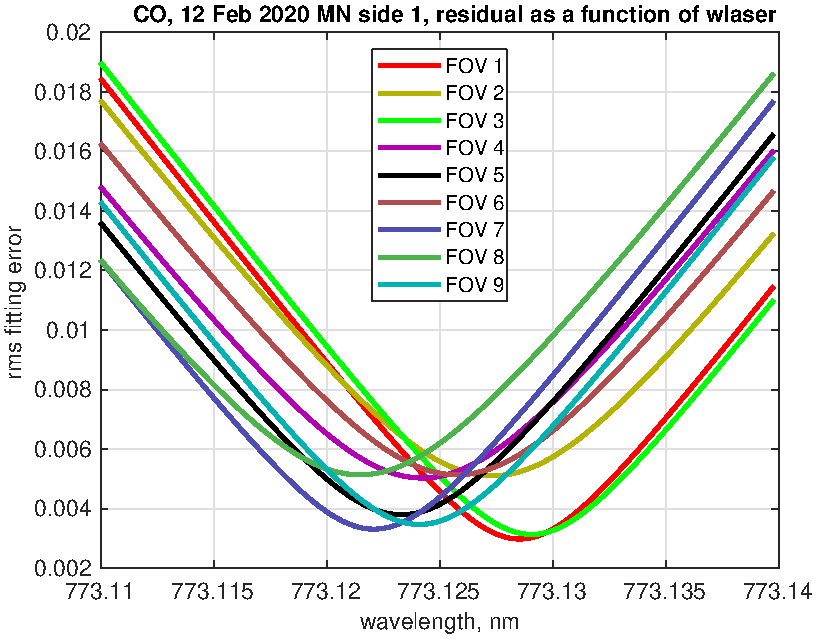
\includegraphics[width=\textwidth]{02-12_mn_s1_CO/CO_wlaser_fit.pdf}
  \end{centering}\vspace{3mm}

Residuals $\rms(a\cdot\tauobs + b - \taucal)$ \\ over the fitting
interval as a function \\ of metrology laser wavelength.

\end{column}
\begin{column}{0.5\textwidth}  
  \begin{centering}
  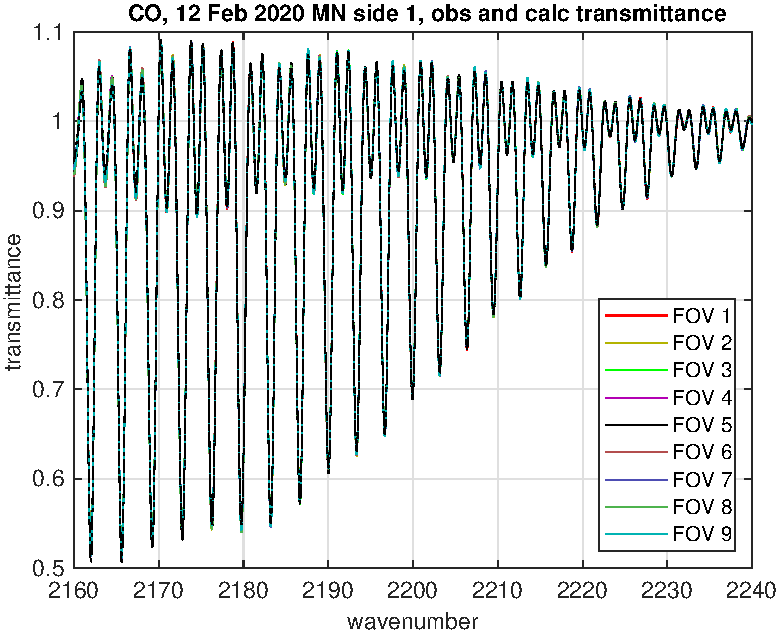
\includegraphics[width=\textwidth]{02-12_mn_s1_CO/CO_obs_and_calc.pdf}
  \end{centering}\vspace{3mm}

Fitted observed and calculated transmittance, over the fitting
interval.  At this level of detail we see all values are very close.

\end{column}
\end{columns}
\end{frame}
%----------- slide --------------------------------------------------%
\begin{frame}
\frametitle{CO side 1 obs minus calc breakouts}
\begin{columns}[t]
\begin{column}{0.5\textwidth}
  \begin{centering}
  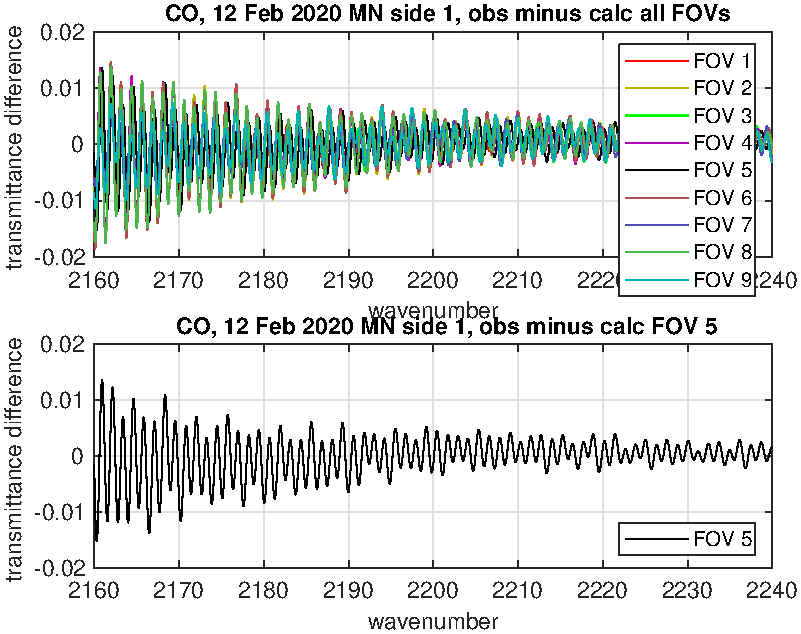
\includegraphics[width=\textwidth]{02-12_mn_s1_CO/CO_breakout_1.pdf}
  \end{centering}\vspace{3mm}

Fitted observed minus calculated transmittance for all FOVs and for FOV~5
alone, over the fitting interval.

\end{column}
\begin{column}{0.5\textwidth}  
  \begin{centering}
  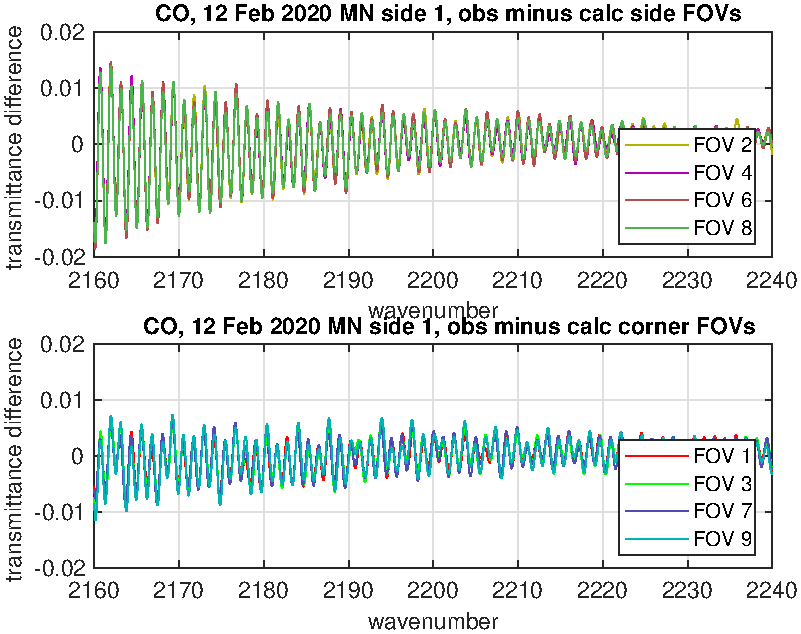
\includegraphics[width=\textwidth]{02-12_mn_s1_CO/CO_breakout_2.pdf}
  \end{centering}\vspace{3mm}

Fitted observed minus calculated transmittance for side and corner FOVs,
over the fitting interval.

\end{column}
\end{columns}
\end{frame}
%----------- slide --------------------------------------------------%
\begin{frame}[fragile]
\frametitle{CO side 1 tabulated residuals}

  metrology laser absolute residuals, ppm
\begin{semiverbatim}\scriptsize
      2.97     5.82    11.25         7   4   1
      2.20     4.53     9.70         8   5   2
      5.56     7.76    12.03         9   6   3
\end{semiverbatim}

  metrology laser relative residuals, ppm
\begin{semiverbatim}\scriptsize
     -1.55     1.29     6.73         7   4   1
     -2.33     0.00     5.17         8   5   2
      1.03     3.23     7.50         9   6   3
\end{semiverbatim}

  regression fitting weights and residuals
\begin{semiverbatim}\scriptsize
 FOV   "a"       "b"     dmin     wmin      wfov
  1   0.989    0.0126   0.0030    11.25   773.1285 
  2   0.991    0.0104   0.0051     9.70   773.1273 
  3   0.989    0.0126   0.0031    12.03   773.1291 
  4   0.993    0.0082   0.0050     5.82   773.1243 
  5   0.989    0.0122   0.0038     4.53   773.1233 
  6   0.994    0.0070   0.0051     7.76   773.1258 
  7   0.992    0.0092   0.0033     2.97   773.1221 
  8   0.997    0.0042   0.0051     2.20   773.1215 
  9   0.987    0.0136   0.0035     5.56   773.1241 
\end{semiverbatim}

\end{frame}
%----------- slide --------------------------------------------------%
\begin{frame}[fragile]
\frametitle{TVAC ILS residual summary}

  metrology laser residuals, ppm
\begin{semiverbatim}\footnotesize
                                             FOV
     Test          1      2      3      4      5      6      7      8      9
01-07\_pl\_s1\_CH4   7.90   8.42  13.60   2.72   5.05   8.94  -0.52   0.78   5.05
01-07\_pl\_s1\_CO2   7.51   9.46  11.40   2.85   5.70   7.90  -2.59  -2.85   1.42
01-08\_pl\_s1\_CO   10.36   8.81  12.18   4.40   4.40   7.77   1.94   1.68   6.22
01-12\_ph\_s1\_CO2  11.37   8.65  10.20   5.94   5.42   3.62  -2.20  -2.97  -3.62
01-13\_ph\_s1\_CH4  11.75   9.69  11.62   6.07   7.23   6.46   1.94   0.26   1.42
01-13\_ph\_s1\_CO   14.85  12.01  12.66   8.14   5.81   7.23   3.62   1.68   3.49
01-19\_ph\_s2\_CO2  14.96  12.00  14.32   9.29   9.16   8.00   2.06   1.55   1.16
02-05\_mn\_s2\_CO2  11.63  11.24  14.08   5.17   7.11   8.91  -1.42  -0.78   0.52
02-11\_mn\_s1\_CH4   8.15   8.02  11.90   3.49   5.56   7.24   0.65   0.26   3.36
02-11\_mn\_s1\_CO2   8.15   8.15  11.12   4.01   4.92   6.47  -2.33  -2.20   0.39
02-12\_mn\_s1\_CO   11.25   9.70  12.03   5.82   4.53   7.76   2.97   2.20   5.56
\end{semiverbatim}

\end{frame}
%----------- slide --------------------------------------------------%
\begin{frame}
\frametitle{Conclusions}
\begin{itemize}

  \item We have done a preliminary analysis of the MN Plateau 22
    CH$_4$, CO$_2$, and CO gas cell tests, and compared these with
    calculated reference truth.  Overall, the results look quite
    good.

  \item The HTBB drift seen in many of the test legs is significant
    but managable with our approach to regression fitting.   The effect
    of the drifts could be reduced with more careful subsetting, if
    needed.

  \item Metrology laser relative residuals are in reasonable
    agreement, and can be reduced further with focal plane
    adjustments.  Metrology laser absolute residuals could be
    reduced with a more judicious choice of neon wavelengh, or 
    possibly by simply using the eng neon value.

\end{itemize}
\end{frame}
%----------- slide --------------------------------------------------%

\end{document}

